\subsection{Interfaces Hommes Machine}

\subsubsection{Généralités}

Le Testeur peut interagir avec PSC par l'IHM présent sur E\_Ecran.
Le Démonstrateur peut interagir avec PSC par les IHM présentes sur AOP et sur E\_Ecran.
PSC peut envoyer des informations aux utilisateurs par l’intermédiaire des écrans et de LEDs de la Board.
Ce dossier de Spécification prend en compte la possibilité d'utiliser différentes langues pour l'affichage sur les différents écrans. 
Il est convenu avec le client que les langues suivantes sont livrés : le français et l'anglais.
À titre d'illustration, seuls les menus en français sont présentés dans ce dossier de spécification.

\subsubsection{Les actions utilisateur}

Les actions possibles du Testeur et du Démonstrateur (interfaces avec les acteurs) sont données en chapitre 2.2.2.2, page \pageref{ContexteLogique}.

\subsubsection{Les écrans}

\paragraph{Vue générale}

La figure \ref{IHMtest1}, page \pageref{IHMtest1}, représente les navigations possibles entre les différents écrans proposés par l’IHM. 
Ces enchaînements sont représentés par un diagramme d'état transition UML. 
La figure \ref{IHMtest}, page \pageref{IHMtest} rappelle les principaux concepts du diagramme d'état transition UML et leur représentation graphique. \\

\begin{figure} [H]
    \centering
    \includegraphics[width=\textwidth]{explications_diagramme_transitions}
    \caption{Légende d'un diagramme UML}
    \label{IHMtest}
\end{figure}

Chaque écran est représenté par un état (rectangle arrondi sur la figure ci-dessus). 
Les transitions entre les écrans représentent une navigation d’un écran à l’autre en précisant l'évènement logique du contexte qui active la transition. 
Cela correspond généralement à des actions faites par l’utilisateur sur les boutons logiciels présents sur l’écran, pour générer l’évènement correspondant.

\begin{figure} [H]
    \centering
    \includegraphics[width=\textwidth]{IHM_connexion_v1}
    \caption{Machine à états des écrans de connexion de l’IHM Android }
    \label{IHMtest1}
\end{figure}

La sphère noire sur la figure n°\ref{IHMtest1} représente l’état initial de création, ici de l’IHM. 
Au lancement du système, « \hyperlink{EcranDemarrage}{Écran\_Démarrage} » s'affiche. 

Puis, après la saisie des informations de connexion, la Pop-Up « \hyperlink{popUpAttenteConnexion}{PopUP\_Attente\_Connexion}~» affiche un message d’attente. 
Ensuite trois affichages sont possibles : 
\begin{itemize}
    \item[\textbf{-}] La Pop-Up « \hyperlink{popUpErreurMDPAdmin}{PopUp\_Erreur\_MDP\_Admin}~» : elle s'affiche si la connexion a été établie mais que le \hyperlink{mdp}{{\textit{mot de passe}}} est erroné.
    \item[\textbf{-}] La Pop-Up « \hyperlink{popUpErreurConnexion}{PopUp\_Erreur\_Connexion}~» : elle s'affiche si, après un temps \hyperlink{tac}{{\textit{TAC}}}, la connexion n'a toujours pas été établie.
    \item[\textbf{-}] L’écran « \hyperlink{EcranAccueil}{Écran\_Accueil} » : il s'affiche lorsque la connexion a été établie et que le \hyperlink{mdp}{{\textit{mot de passe}}} est correct.
\end{itemize}
Ce dernier est considéré comme un « super-état » et est détaillé dans le prochain paragraphe.

\hypertarget{MaEHome}{}
\begin{figure} [H]
    \centering
    \includegraphics[width=\textwidth]{IHM_root_v1}
    \caption{Machine à états des écrans de navigation de l’IHM Android}
    \label{IHMtest2}
\end{figure}

La sphère noire sur la figure n°\ref{IHMtest2} représente la suite de l’enchaînement entre les écrans, ici des écrans de navigation, après que la connexion ait été établie. 
À la suite de cette connexion, l’écran «~\hyperlink{EcranAccueil}{Écran\_Accueil} » est affiché.
Cet écran est un écran de transition, qui permet au Démonstrateur de se déplacer dans les quatre écrans suivants : « \hyperlink{EcranListe}{Écran\_Liste} », « \hyperlink{EcranCalendrier}{Écran\_Calendrier} », «~\hyperlink{EcranVideo}{Écran\_Vidéo} », et « \hyperlink{EcranPorte}{Écran\_Ouverture\_Porte} ».
Il peut également passer à l’état final (l’arrêt de l’application), représenté par le cercle contenant une sphère noire sur la figure \ref{IHMtest1}.

Les écrans « \hyperlink{EcranCalendrier}{Écran\_Calendrier} » et « \hyperlink{EcranVideo}{Écran\_Vidéo} » affichent des informations à titre consultatif pour le Démonstrateur.
En cas d'arrêt de la réception du \hyperlink{video}{\textit{flux vidéo}} (via l'évènement videoIndisponible()), la Pop-Up d’avertissement « \hyperlink{popUpVideoIndisponible}{PopUp\_VideoIndisponible}~» s'affiche, contraignant le Démonstrateur à retourner à l'«~\hyperlink{EcranAccueil}{Écran\_Accueil} ».

L’écran « \hyperlink{EcranPorte}{Écran\_Ouverture\_Porte} » permet la demande de l’ouverture de la Porte par le Démonstrateur. 

L’écran « \hyperlink{EcranListe}{Écran\_Liste} » permet la consultation et la modification de la liste des employés. 
En cas d’ajout d’un employé, l’écran « \hyperlink{EcranAjoutStandard}{Écran\_Ajout} » s’affiche, et en cas de suppression d’un employé, la Pop-Up d’avertissement « \hyperlink{popUpSuppression}{PopUp\_Suppression}~» s’affiche. 

Les écrans sont détaillés dans les chapitres suivants.

\newpage

% Les écrans de connexion %
\paragraph{Écran Démarrage}
\hypertarget{EcranDemarrage}{}

\begin{figure} [H]
    \centering
    \includegraphics[width=0.4\textwidth]{Ecran_demarrage_android}
    \caption{Écran de démarrage}
    \label{Écran Démarrage}
\end{figure}

L’écran « Écran\_Démarrage » affiche un message d’accueil avec la chaîne de caractères «~Connexion AOP », ainsi que deux zones de texte à remplir.
La première contient l’adresse \hyperlink{IP}{{\textit{IP}}} de la \hyperlink{bd}{{\textit{Board}}}, et la deuxième contient le \hyperlink{mdp}{{\textit{mot de passe}}}. 
Le bouton «~Connexion~» permet de passer à la PopUP « \hyperlink{popUpAttenteConnexion}{PopUP\_Attente\_Connexion} », ce qui correspond à l'évènement « seConnecter(...) ».

\newpage

\paragraph{PopUP attente connexion}
\hypertarget{popUpAttenteConnexion}{}

\begin{figure} [H]
    \centering
    \includegraphics[width=0.4\textwidth]{PopUp_attenteConnexion_android}
    \caption{PopUP attente connexion}
    \label{PopUP attente connexion}
\end{figure}

La Pop-Up « PopUP\_Attente\_Connexion » affiche un message avec la chaîne de caractères « Connexion en cours … ».

Si la connexion est établie, l’écran passe à l’écran « \hyperlink{EcranAccueil}{Écran\_Accueil} ».

Si la connexion est établie mais que la Board indique que le mot de passe est incorrect, alors l'écran affiche la Pop-Up « \hyperlink{popUpErreurMDPAdmin}{PopUp\_Erreur\_MDP\_Admin} ».

Si la connexion n'est pas établie au bout d’un temps \hyperlink{tac}{\textit{TAC}} (Temps d’Attente de Connexion) alors l’écran affiche la Pop-Up « \hyperlink{popUpErreurConnexion}{PopUp\_Erreur\_Connexion} ».

\paragraph{PopUP erreur MDP admin}
\hypertarget{popUpErreurMDPAdmin}{}

\begin{figure} [H]
    \centering
    \includegraphics[width=0.4\textwidth]{PopUp_erreurMDP_android}
    \caption{PopUP erreur MDP admin}
    \label{PopUP erreur MDP admin}
\end{figure}

La Pop-Up « PopUp\_Erreur\_MDP\_Admin » affiche un message avec la chaîne de caractères « Erreur mot de passe ». 
Le bouton « Return » renvoie à l’écran de démarrage, ce qui correspond à l'évènement « return() ».

\paragraph{PopUP erreur connexion}
\hypertarget{popUpErreurConnexion}{}

\begin{figure} [H]
    \centering
    \includegraphics[width=0.4\textwidth]{PopUp_erreurConnexion_android}
    \caption{PopUP erreur connexion}
    \label{PopUP erreur connexion}
\end{figure}

La Pop-Up « PopUp\_Erreur\_Connexion » affiche un message avec la chaîne de caractères «~Erreur de connexion ».
Le bouton « Return » renvoie à l’écran de démarrage, ce qui correspond à l'évènement « return() ».

\paragraph{Écran Accueil}
\hypertarget{EcranAccueil}{}

\begin{figure} [H]
    \centering
    \includegraphics[width=0.4\textwidth]{Ecran_accueil_android}
    \caption{Écran d'accueil}
    \label{Ecran d'accueil}
\end{figure}

L’écran « Écran\_Accueil », affiche 5 boutons, qui permettent la navigation dans l’application.
\begin{itemize}
    \item[\textbf{-}]	Le bouton « Employés », permet d’afficher l’écran « \hyperlink{EcranListe}{Écran\_Liste} », ce qui correspond à l'évènement « demanderListeEmployés() » sur la \hyperlink{MaEHome}{\textit{MàE des écrans de navigation de l’IHM Android}}.  
    \item[\textbf{-}]	Le bouton « Calendrier », permet d’afficher l’écran « \hyperlink{EcranCalendrier}{Écran\_Calendrier} », ce qui correspond à l'évènement « demanderCalendrier(...) ».
    \item[\textbf{-}]	Le bouton « Vidéo », permet d’afficher l’écran « \hyperlink{EcranVideo}{Écran\_Vidéo} », ce qui correspond à l'évènement « demanderVidéo() ».
    \item[\textbf{-}]	Le bouton « Contrôle porte », permet d’afficher l’écran « \hyperlink{EcranPorte}{Écran\_Ouverture\_Porte}~», ce qui correspond à l'évènement « demanderContrôlePorte() ».
    \item[\textbf{-}]	Le bouton « Quitter », permet la fermeture de l’application, ce qui correspond à l'évènement « quitterAOP() ».
\end{itemize}

\paragraph{Écran Liste}
\hypertarget{EcranListe}{}

\begin{figure} [H]
    \centering
    \includegraphics[width=0.4\textwidth]{Ecran_liste_android}
    \caption{Écran liste des employés}
    \label{Écran liste des employés}
\end{figure}

%« Implémenté lors de l’incrément 2 »

L’écran « Écran\_Liste » permet l’affichage de l’ensemble des employés enregistrés dans \hyperlink{donneesTesteurs}{\textit{Données\_Testeurs}}.

Pour chaque employé est visible son nom, son prénom, et son \hyperlink{rol}{\textit{rôle}}.
Le bouton « Ajouter nouvel employé » renvoie vers l’écran « \hyperlink{EcranAjoutStandard}{Écran\_Ajout} », ce qui correspond à l'évènement «~demanderAjoutEmployé()~», présent sur la \hyperlink{MaEHome}{\textit{MàE des écrans de navigation de l'IHM Android}}.

Les boutons représentés par une croix, à côté de chaque nom des employés, renvoient vers la Pop-up « \hyperlink{popUpSuppression}{PopUp\_Suppression} », ce qui correspond à l'évènement « demanderSuppressionEmployé(...) ».

Le bouton « Return » en haut à gauche renvoie vers l’écran précédent, ce qui correspond à l'évènement « return() ». 

\paragraph{Écran ajout employé (standard)}
\hypertarget{EcranAjoutStandard}{}

\begin{figure} [H]
    \centering
    \includegraphics[width=0.4\textwidth]{Ecran_ajoutStandard_android}
    \caption{Écran ajout employé (standard)}
    \label{Écran ajout employé (standard)}
\end{figure}

\paragraph{Écran ajout employé (spécial)}
\hypertarget{EcranAjoutSpecial}{}

\begin{figure} [H]
    \centering
    \includegraphics[width=0.4\textwidth]{Ecran_ajoutSpecial_android}
    \caption{Écran ajout employé (spécial)}
    \label{Écran ajout employé (spécial)}
\end{figure}

%« Implémenté lors de l’incrément 2 »

Dans le premier onglet « Nom », le Démonstrateur doit saisir le \hyperlink{nom}{\textit{nom}} de l'employé. 
Dans le deuxième onglet « Prénom », le Démonstrateur doit saisir le \hyperlink{prénom}{\textit{prénom}} de l'employé.
Ces deux saisies doivent respecter des \hyperlink{caracEmploye}{\textit{caractéristiques}} de nommage.
Le bouton « Importer une image » dans la partie « Photo » permet au Démonstrateur d’importer une \hyperlink{photo}{\textit{photo}} de l'employé, photo utilisée pour la reconnaissance faciale.
Un appui sur ce bouton correspond à l'évènement « importerImage(...)~».

L’onglet « Rôle » permet la sélection du \hyperlink{rol}{\textit{rôle}} de l’employé parmi la liste prédéfinie.
En cas de la sélection du rôle « Employé spécial », de nouvelles fonctionnalités se déverrouillent permettant au Démonstrateur de personnaliser les \hyperlink{hor}{\textit{horaires}} d’accès du nouvel employé.
Le bouton « CONFIRMER » enregistre les données du nouvel employé dans \hyperlink{donneesTesteurs}{\textit{Données\_Testeurs}}, et renvoie vers l’écran « \hyperlink{EcranListe}{Écran\_Liste} », ce qui correspond à l'évènement « confirmer() ».
Le bouton «~ANNULER » n’enregistre pas les données du nouvel employé dans \hyperlink{donneesTesteurs}{\textit{Données\_Testeurs}}, et renvoie vers l’écran « \hyperlink{EcranListe}{Écran\_Liste} », ce qui correspond à l'évènement « annuler() ».

\paragraph{PopUp suppression}
\hypertarget{popUpSuppression}{}

\begin{figure} [H]
    \centering
    \includegraphics[width=0.4\textwidth]{PopUp_suppressionEmploye_android}
    \caption{PopUp suppression employés}
    \label{PopUp suppression employés}
\end{figure}

La Pop-Up « PopUp\_Suppression » affiche le nom et le prénom de l’employé à supprimer, ainsi que deux boutons. 
Le bouton « CONFIRMER » permet la suppression des données de l’employé présélectionné et renvoie vers l’écran « \hyperlink{EcranListe}{Écran\_Liste} », ce qui correspond à l'évènement « confirmer() ». 
Le bouton « ANNULER » renvoie à l’écran « \hyperlink{EcranListe}{Écran\_Liste} » sans supprimer de données, ce qui correspond à l'évènement « annuler() ».

\paragraph{Écran calendrier}
\hypertarget{EcranCalendrier}{}

\begin{figure} [H]
    \centering
    \includegraphics[width=0.4\textwidth]{Ecran_calendrier_android}
    \caption{Écran calendrier}
    \label{Écran calendrier}
\end{figure}

L’écran « Écran\_Calendrier » permet l’affichage du calendrier d’un seul employé à la fois. 
L'onglet de sélection, situé en haut, permet de choisir le calendrier d'un employé parmi ceux de \hyperlink{donneesTesteurs}{\textit{Données\_Testeurs}}.
%Inc
%Lors de l'incrément 1, la BdD\_Testeurs n'est pas livré, les \hyperlink{caracEmploye}{\textit{informations des employés}} sont codées en durs.
Par défaut lorsque le Démonstrateur affiche l'écran, aucun employé n'est sélectionné et le calendrier est vide. 

La navigation dans le calendrier se fait via des déplacements sur l’écran tactile du support de l’application.

Sur le calendrier, apparaissent les heures d’accès pour l’employé sélectionné. 
L’affichage du calendrier se fait par créneaux \hyperlink{hor}{\textit{horaires}}.
Le bouton « Return » en haut à gauche renvoie vers l’écran précédent, ce qui correspond à l'évènement « return() », sur la \hyperlink{MaEHome}{\textit{MàE des écrans de navigation de l’IHM Android}}. 

\paragraph{Écran ouverture de la Porte}
\hypertarget{EcranPorte}{}

\begin{figure} [H]
    \centering
    \includegraphics[width=0.4\textwidth]{Ecran_porte_android}
    \caption{Écran ouverture de la Porte}
    \label{Écran ouverture de la porte}
\end{figure}

%« Implémenté lors de l’incrément 2 »

L’écran « Écran\_Ouverture\_Porte » permet l’affichage de l'état de la Porte et de contrôler l'ouverture de la Porte à distance.

En haut de l’écran, l’état de la Porte est affiché, cet état est représenté par deux couleurs : le rouge pour l’état fermé et le vert pour l’état ouvert.
Juste en-dessous, le bouton « Déverrouiller la porte » permet le \hyperlink{deverrouiller}{\textit{déverrouillage}} de la Porte à distance, ce bouton correspond à l'évènement «~demanderOuverturePorte() ».

Le bouton « Return », en haut à gauche, renvoie vers l’écran précédent, ce bouton correspond à l'évènement « return() ».

\paragraph{Écran de la vidéo}
\hypertarget{EcranVideo}{}

\begin{figure} [H]
    \centering
    \includegraphics[width=0.4\textwidth]{Ecran_video_android}
    \caption{Écran de la vidéo}
    \label{Écran de la vidéo}
\end{figure}

L’écran « Écran\_Vidéo », permet l’affichage en temps réel de la \hyperlink{video}{\textit{vidéo}} filmée par E\_Caméra. 
Le bouton « Return » en haut à gauche renvoie vers l’écran précédent, ce qui correspond à l'évènement « return() ». 

\newpage

\paragraph{PopUp Vidéo Indisponible}
\hypertarget{popUpVideoIndisponible}{}

\begin{figure} [H]
    \centering
    \includegraphics[width=0.4\textwidth]{PopUp_videoIndisponible_android}
    \caption{PopUp vidéo Indisponible}
    \label{PopUp vidéo Indisponible}
\end{figure}

La Pop-Up « PopUp\_VideoIndisponible » indique au Démonstrateur que SoftSonnette a stoppé l'envoie en continue de la vidéo.
Le bouton « Return » en haut à gauche renvoie vers l’écran précédent, ce qui correspond à l'évènement « return() ». 

\newpage

\paragraph{Écran SoftSonnette}
\hypertarget{EcranWebcamConnec}{}

\begin{figure} [H]
    \centering
    \includegraphics[width=0.7\textwidth]{EcranSonnette_webCamConnecte_c}
    \caption{Écran de la sonnette avec E\_Caméra connectée}
    \label{Écran de la sonnette webCam connectée}
\end{figure}

\paragraph{Écran SoftSonnette [Erreur Communication]}
\hypertarget{EcranErreurCommunication}{}

\begin{figure} [H]
    \centering
    \includegraphics[width=0.7\textwidth]{EcranSonnette_erreur_com_C}
    \caption{Écran de la sonnette affichant qu'une erreur de communication avec SoftPorte est survenue}
    \label{Écran de la sonnette affichant qu'une erreur de communication avec SoftPorte est survenue}
\end{figure}

\paragraph{Écran SoftSonnette [Erreur E\_Caméra Non Connectée]}
\hypertarget{EcranWebcamNonConnec}{}

\begin{figure} [H]
    \centering
    \includegraphics[width=0.7\textwidth]{EcranSonnette_webCamNonConnecte_c}
    \caption{Écran de la sonnette avec E\_Caméra non connectée}
    \label{Écran de la sonnette webCam non connectée}
\end{figure}

L’écran « Écran\_SoftSonnette », affiche le \hyperlink{video}{\textit{flux vidéo}} filmé par E\_Caméra. 
Trois variantes sont présentes sur cet écran: \\
\begin {itemize}
    \item Lorsque tout est en état de marche, le flux est affiché dans le cadre dédié.
    \item Lorsque l'initialisation de la communication entre SoftSonnette et SoftPorte échoue, la chaîne de caractères suivante s'affiche : « Erreur communication SoftPorte ».
    \item Lorsqu'aucun \hyperlink{video}{\textit{flux vidéo}} n'est disponible (E\_Caméra non connectée) la chaîne de caractères suivante s'affiche : « Webcam non connectée ».
\end{itemize}
Sur toutes les variantes sont présents deux boutons et un voyant représentant l'état de la Porte.

En bas à gauche se trouve l'état actuel de la Porte (voyant vert = Porte ouverte et voyant rouge = Porte fermé).
Le bouton « Quitter » permet l'arrêt de SoftSonnette, ce qui correspond à l'évènement « quitterSoftSonnette() ». 
Le bouton « Sonner » demande à SoftSonnette la permission de rentrer, ce qui correspond à l'évènement « sonner() ».

\paragraph{Vue Board}
\hypertarget{EcranSoftPorte}{}

\begin{figure} [H]
    \centering
    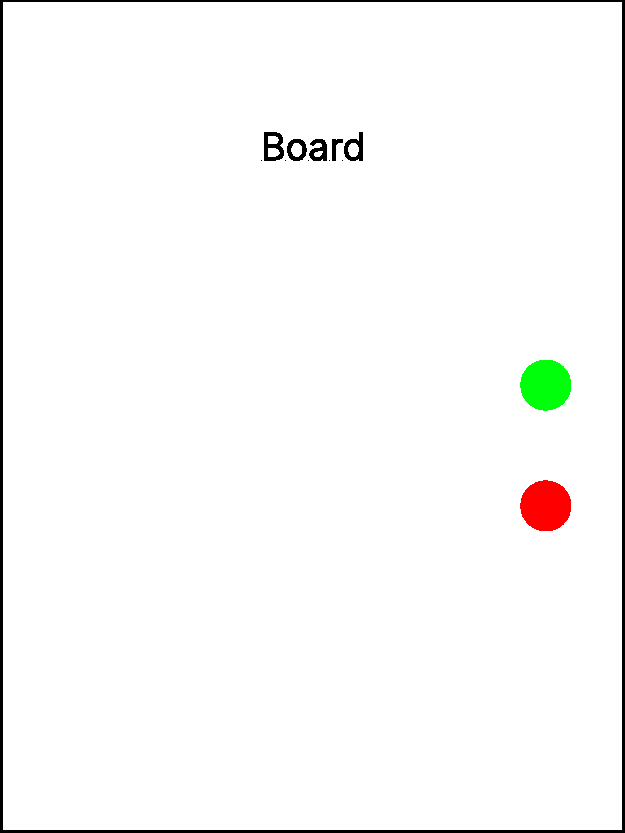
\includegraphics[width=0.4\textwidth]{LedSoftPorte}
    \caption{Vue Board}
    \label{Vue Board}
\end{figure}

La LED LD5 située sur la Board s'allume en vert afin de signaler le bon fonctionnement de SoftPorte. 
S'il y a eu un démarrage incorrect la LED ne s'allume pas.

La LED LD6 située sur la Board s'allume en rouge si le visage du Testeur n'est pas reconnu.
Si le visage est reconnu la LED ne s'allume pas. 
